\documentclass[tikz]{standalone}
\usepackage{fontspec}
\renewcommand*{\familydefault}{\sfdefault}
\usepackage{standalone}
\usetikzlibrary{decorations.pathreplacing}
\usetikzlibrary{arrows.meta, decorations.pathreplacing, shapes.geometric}
\usetikzlibrary{bayesnet}

\begin{document}
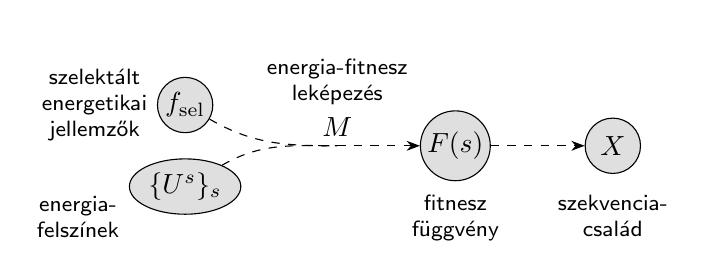
\begin{tikzpicture}[every node/.style={draw, shape=circle, fill=gray!30!white}]
% Define nodes
\path (0,0)
node[obs] (X) {\(X\)}
(X) +(0:-2.0 cm) node[obs] (fitness) {\(F(s)\)}
(fitness) +(180:1.5 cm) coordinate (fuse)
(fitness) +(90:1.5 cm)
%node[anchor=south, shape=rectangle, align=center, font=\footnotesize, rounded corners] (mech) {evolutionary\\mechanisms}
(fuse) to
+(15:-2.0 cm)
node[obs, shape=ellipse] (U) {\(\{U^s\}_s\)}
to
+(-15:-2.0 cm)
node[obs] (fsel) {\(f_\mathrm{sel}\)}
(fuse) +(90:0.0 cm) node[draw=none, fill=none, anchor=south, shape=rectangle] (map) {\(M\)}
;

\draw[dashed] (U) to[out=30, in=180] (fuse);
\draw[dashed] (fsel) to[out=-30, in=180] (fuse);
\draw[-Stealth, dashed] (fuse) -- (fitness); 
\draw[-Stealth, dashed] (fitness) -- (X); 

\path[every node/.style={draw=none}, font=\footnotesize]
(X) +(-90:0.5 cm) node[anchor=north, align=center] {szekvencia-\\család}
(fitness) +(-90:0.5 cm) node[anchor=north, align=center] {fitnesz\\függvény}
(U.west) node[anchor=north east, align=center] {energia-\\felszínek}
(fsel.west) node[anchor=east, align=center]
{szelektált\\energetikai\\jellemzők}
(map) +(90:0.15 cm) node[anchor=south, align=center] {energia-fitnesz\\leképezés}
;

\end{tikzpicture}

\end{document}



